\section{Solution Approach}

% to add / extend - solution approach -> Section 1.3 
% -> how could we solve these issues and -> Section 1.3
% begründung für blockchain - slide skizze von prof stiller bcoln vorlesung

From the stated problem the question arises what technology should be used to manage these. Based on the work of \citet{wust2018you} and the solution concept discussed in following subsection, a permissionless BC is suitable.

\subsection{Solution Concept}\label{chapter:introduction:concept}
% kurze übersicht zu unserem approach - und dann weiter mit genaueren infos zu blockchain und allg background
Figure \ref{fig:dlt-based-landscape1} shows a conceptual overview of the distributed ledger technology (DLT) based architecture. The distributed ledger (DL) handles storage and distribution of the digital assets (tickets) and builds the core logic in the system. All transactions, e.g. creation of events or buying tickets, are handled through a set of SCs. This approach enables anyone to build a graphical user interface (GUI) for invoking the SCs. This is even encouraged through paying a small fraction of each interaction with a GUI to the \textit{GUI Builder}. The same payout technique is applied for people promoting an event which allows for transparent promotion contract with instant payout between event hosts and public figures. In order to enable personalized tickets for a controlled aftermarket, \textit{ID approvers} can register themselves on the BC and offer their service to event hosts. This is again incentivised by providing a payout every time a guest, that was approved by them, buys a ticket. Event guests are then able to register themselves with the required ID approver for their event of interest and buy tickets through their GUI of choice. They can also resell their ticket or buy tickets from the aftermarket directly on the BC.
\begin{figure}[H]
    \centering
    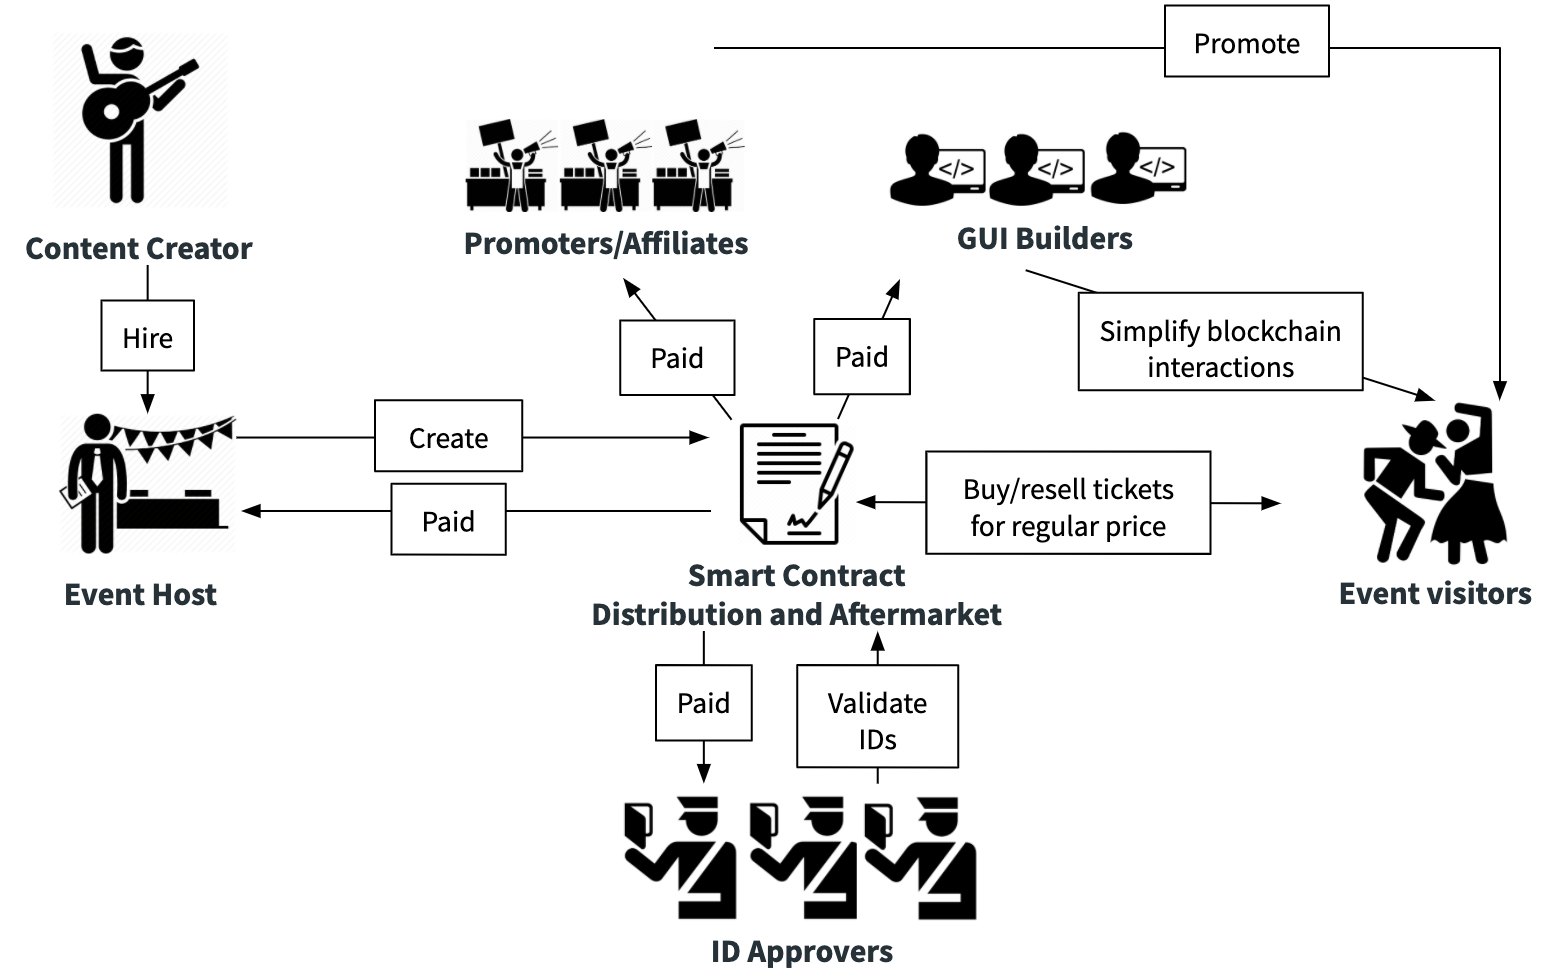
\includegraphics[width=16cm]{figures/dlt-based-landscape.png}
    \caption{DLT-based architecture}
    \label{fig:dlt-based-landscape1}
\end{figure}

\subsection{Additionally Stakeholders}
% new generated stakeholders like GUI Builders

The stakeholder described in Section \ref{chapter:introduction:Stakeholder} are still present in the suggested solution described in Section \ref{chapter:introduction:concept}.
However, this proposed solution also introduces two additional stakeholders. These are characterized as following.

\subsubsection{GUI Builder}
GUI Builders are entities, that provide a GUI, that enables event guests to interact with the Ethereum BC in a simple way. They spend time and money to develop, host and maintain this connection. Therefore, their main goal is to earn funds, whenever a guest is using their GUI to interact with the DL. Since the GUI Builder only earns funds, whenever his GUI is used, he is incentivised to create the best GUI, to have all the guest using his platform.

\subsubsection{ID approvers}
ID approvers are entities, that verify, whether the guest has control over an identity he claimed to be his. Their main goal is to earn funds by approving the identities of guest. They do this, whenever a guest buys a ticket, that requires the guest to be approved by this specific ID approver. Therefore, they want to establish themselves as a trusted and efficient approver, to have event hosts use them as their ID approver for their events.
